\documentclass[12pt]{article}
\usepackage{fullpage}
\usepackage{graphicx}
\usepackage{hyperref}
\usepackage{amssymb}
\usepackage{bm}

\def\lesim{\ \hbox to 0 pt{\raise .6ex\hbox{$<$}\hss} \lower.5ex\hbox{$\sim$}\ }

\title{Plasma electrostatic wave dispersion solution for arbitrary ion
  distributions} \author{I.H.~Hutchinson}

\begin{document}
\maketitle

\begin{abstract}
A method is described to solve numerically the dispersion relation and hence
investigate stability of arbitrary ion distributions to longitudinal
electrostatic oscillations in the ion-acoustic range of velocities.
Several subtleties arise that are bypassed in the historic analytic
treatments. A dimensionless formulation is implemented that gives
robust graphical interpretation and allows direct solution and
intuitive display. It is applied to a range of different electrostatic
waves and instabilities. 
\end{abstract}

\section{Background Theory}

The longitudinal relative susceptibility to linear waves
($\propto \exp i({\bm k.\bm x}-\omega t)$) that are presumed to have real
wave-vector ${\bm k}$ and possibly complex frequency $\omega$, for a
uniform unmagnetized plasma or when the  $\bm k$-direction is parallel
to the magnetic field is
\begin{equation}
\chi=\sum \chi_j\quad \mbox{with}\quad
  \chi_j = -{\omega_{pj}^2\over k^2} \int {\partial
    f_j\over \partial v } {1\over v- v_p} dv
\end{equation}
where $j$ denotes the species, $q_j=Z_je$ is its charge, $n_j$ its
density, $\omega_{pj}^2=n_j q_j^2/\epsilon_0 m_j$ its plasma frequency
squared, $v$ the velocity in the parallel (${\bf k}$) direction, $f_j$
the \emph{normalized} one-dimensional parallel velocity distribution
function (such that $\int f_j dv=1$), and $v_p$ is the phase velocity
\begin{equation}
  \label{eq:phasevel}
  v_p\equiv \omega/k.
\end{equation}
The integral must be performed using the standard Landau
prescription along a contour below the pole at $v_p$ in the complex
$v$-plane.

It is convenient to introduce an energy scale expressed as an
effective temperature $T_0$. In terms of this temperature, the Debye
length is $\lambda_{D} = \sqrt{\epsilon_0 T_0/e^2 n_e}$ and the sound
speed is $c_{s} = \sqrt{T_0/m_i}$. At this stage one can think of these as
corresponding to electron temperature $T_e=T_0$ and ion mass
$m_i$. However, we will later sometimes consider $T_e$ to be variable,
independent of $T_0$. In terms of these energy scaled parameters we
can write
\begin{equation}\label{ionint}
  k^2\lambda_{D}^2 \chi_j = -  Z_j^2 {m_i\over m_j} c_{s}^2 \int  {\partial
    f_j\over \partial v } {1\over v- v_p} dv\ .
\end{equation}
We note that the right hand side of this expression, for given plasma
parameters, is a function only of the complex phase velocity $v_p$,
not of $k$ and $\omega$ independently. Expressed in this way, we can
see that the dispersion relation is determined by the sum of
distribution functions (differentiated and) multiplied by $Z_j^2/m_j$
integrated over a single velocity space. One can illustrate this
\begin{figure}[htp]
  \centering
  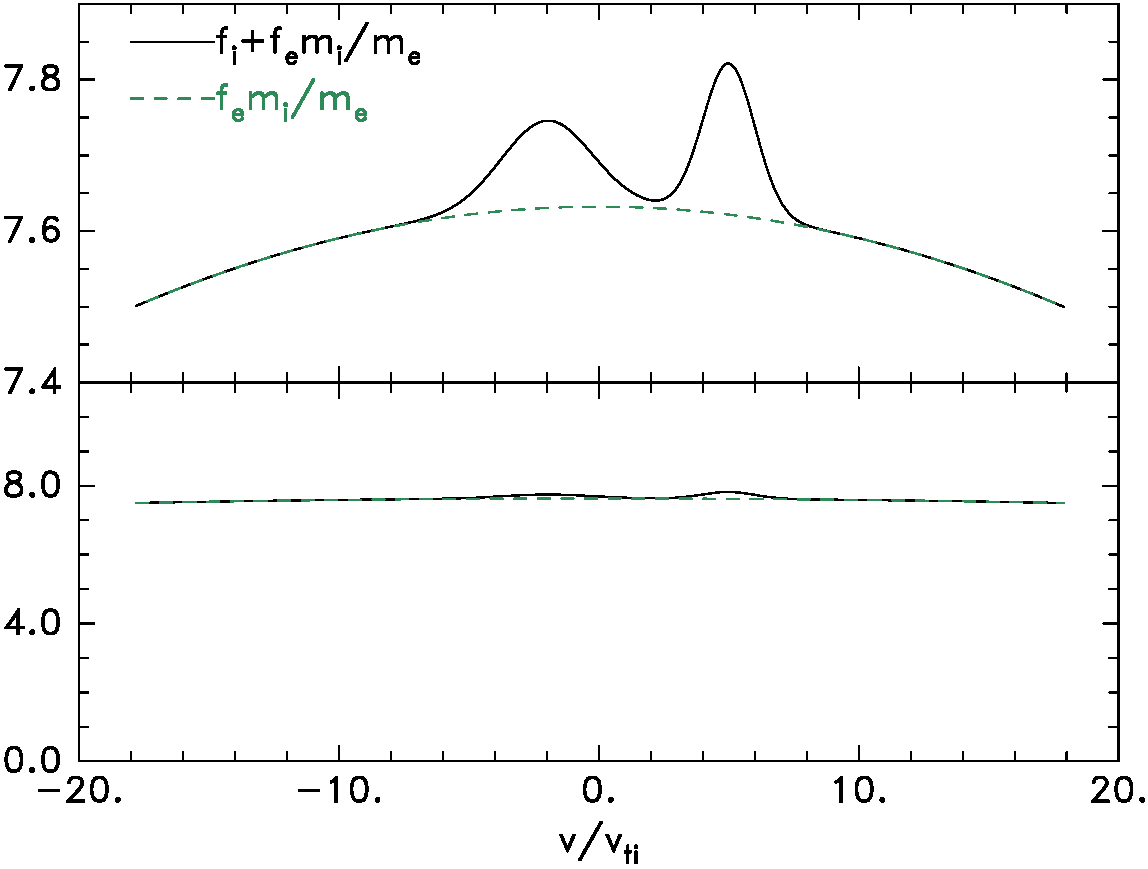
\includegraphics[width=0.6\hsize]{combined}
  \caption{Combined velocity distribution weighted by $1/m_j$, which
    could be used to determine stability by the Penrose criterion.}
  \label{fig:penrose}
\end{figure}
by plotting the sum of the distributions so weighted. An example is
Fig.\ \ref{fig:penrose}. It has been plotted twice; the lower panel
avoids the suppressed zero of the upper panel, so as to emphasize the
fact that the ion susceptibility arises as a small perturbation on top
of a nearly flat electron contribution. The stability of the combined
distribution $f_c(v)=f_i(v)+ f_e(v)m_i/m_e$ could be analysed by the
Penrose criterion, namely that there are unstable modes if and only if
there exists a real $v_m$ such that $f_c(v_m)$ is a (local)
minimum and $\int[f_c(v)-f_c(v_m)]/(v-v_m)^2 dv>0$. The integral
condition amounts to requiring the local minimum to be deep enough
compared with the surrounding distribution. In the context of ion-ion
instabilities, one can see that the higher the central $f_e$ is, the
less relatively deep a given ion distribution minimum is. Thus lower
electron temperature (which makes $f_e$ higher) tends to stabilize the
combined distribution. This effect is \emph{not} a result of electron Landau
damping.  We develop here a way to to understand the problem more
quantitatively, yet still giving an intuitive graphical rendering in
velocity space.

The dispersion relation for (electrostatic) longitudinal waves is 
\begin{equation}
  \epsilon = 1 + \chi =0 \ ,\ \mbox{\quad or\quad} \chi =-1\ .
\end{equation}
Solving it can be approached by finding those phase velocities $v_p=\omega/k$
for which the imaginary part of $ k^2\lambda_{D}^2\chi$ (and hence of
$\chi$) vanishes. If the corresponding real part, denoted
$\Re ( k^2\lambda_{D}^2\chi)$, for those $v_p$ is negative, then there
exists a real $k$ for which $\Re (\chi)=-1$ and the dispersion
relation is solved. However, for $v_p$ such that
$\Re(k^2\lambda_{D}^2\chi)>0$, no solution exists. If we are therefore
able to evaluate the integrals to obtain $k^2\lambda_{D}^2 \chi_j$ at
relevant values of $v_p$, the above approach provides an algorithm for
solving the dispersion relation.

In analytic treatments
of this problem, 
convenient analytic representations of the ion distribution functions
are generally used. They provide closed-form expressions for the
integrals, often in terms of the (Fried and Comte) plasma dispersion
function which arises for Gaussian distributions. The present work
addresses the more general problem when the ion distribution functions
are prescribed in arbitrary numerical terms.

\section{Integrating the Susceptibility}

\subsection{Electron Susceptibility}

In principle the electron distribution might be arbitrary as well as
the ion distribution. However, the generally very different velocity
scale of the electron distribution means that for the exploration of
waves in the ion-acoustic frequency range, the electrons' response is
usually defined by the Debye length and the low velocity part of their
distribution. Performing detailed numerical integrals over the
electron distribution is then neither accurate nor appropriate. Therefore
we regard the electrons here as having a Maxwellian distribution. As
is well known, the electron susceptibility integrals can then be
written
\begin{equation}\label{chiefull}
   k^2\lambda_{De}^2 \chi_e = {1\over \sqrt{\pi}} \int {z {\rm
       e}^{-z^2} \ dz\over z-x} =
1 -2xe^{-x^2}\int_0^x e^{z^2}dz + i\sqrt{\pi} x e^{-x^2}
\end{equation}
where $x=\omega/k\sqrt{2T_e/m_e}$; the first integral is along the
Landau contour. It should be emphasized that the Debye length here
$\lambda_{De}$, is evaluated using the actual electron temperature
$T_e$, not the scaling temperature $T_0$ (if it is different). This
expression is an embodiment of the plasma dispersion function. In
terms of standard functions it can be considered the derivative of
$(-i\sqrt{\pi}/2)\exp(-x^2)\mbox{erfc}(-ix)$. In the ion-acoustic
regime with $\bar v_i\simeq \bar v_e$, $\chi_e$ is usually well approximated
by an expansion that takes $v_p$ to be small compared with
$\sqrt{2T_e/m_e}$, which yields
\begin{equation}\label{chie}
   k^2\lambda_{D}^2 {T_e\over T_0} \chi_e=
k^2\lambda_{De}^2 \chi_e \approx 1 + i \sqrt{\pi m_e\over 2 T_e}\; v_p\ .
\end{equation}

For frequencies well below the electron gyro-frequency and
correspondingly small $k \rho_e \ll 1$ (where $\rho_e$ is the thermal
gyro-radius) the one-dimensional expressions can be readily extended
to give the required longitudinal electron susceptibility for oblique
propagation with respect to the magnetic field when the wave-vector
has a component $k_\parallel$ along the magnetic field. Purely
parallel electron motion replaces $f$ with parallel distribution
$f_\parallel$, and replaces speed $v$ with $v_{\parallel}$ (and $v_p$
with $v_{p\parallel}$) in equation (\ref{ionint}) or (\ref{chie}), and
$x=\omega/k_\parallel\sqrt{2T_e/m_e}$ in (\ref{chiefull}). The $k^2$
factor multiplying $\chi_e$, which arises from the Laplacian in
Poisson's equation, remains the total $k$. {Algebraically, the
  electron current along $B$ is
  $j_\parallel = -(q^2i\omega/mk_\parallel^2)\int {df_\parallel\over
    dv_\parallel}{ dv_\parallel\over(\omega/k_\parallel -
    v_\parallel)} E_\parallel$ and the longitudinal components are
  $j_k=(k_\parallel/k) j_\parallel$, $E_k=(k/k_\parallel)E_\parallel$.
  Thus
  $k^2\lambda_{De}^2\chi_{kk}= -\int {df_{e\parallel}\over
    dv_\parallel}/(\omega/k_\parallel - v_\parallel) dv_\parallel$ is
  the longitudinal electron susceptibility contribution.}  This
approximation is appropriate for Lower Hybrid waves and
instability. However, McMillan (2006) says that a term
$(k_\perp/k)^2(\omega_{pe}/\Omega_e)^2$ should be added to the
electron susceptibility to account for incomplete electron
magnetization.


Expansion eq.\ (\ref{chie}) becomes inappropriate for angles that
enhance $v_{p\parallel}$ so much as to violate $|x|\ll 1$. Then a full
numerical implementation of the Faddeeva function,
$\exp(-x^2)\mbox{erfc}(-ix)$, in eq.\ (\ref{chiefull}) must be
used. It is also required for large shifts between the electron and
ion distributions.


\iffalse
The imaginary part of eq.\ (\ref{chie}) represents electron Landau
damping and arises from the contribution of the residue from the pole
after a principal value evaluation of the integral.  This form applies
to an unshifted electron distribution. It defines the frame of
reference as being that in which the electron drift (or more precisely
the peak of the electron distribution) velocity is zero.  For a
non-thermal electron distribution, we can consider eq.\ (\ref{chie})  to be
the lowest significant order terms of a Taylor expansion of $k^2
\chi_e$, and thereby a \emph{definition} of what we mean by
$\lambda_{D}$ and the relative weight of Landau damping, $w_L$. In
other words, we must take $\lambda_{D}$ to be such that
$\lambda_{D}^2 =1/[k^2\Re (\chi_e)] $, $T_e$ then to be $T_e =
\lambda_{D}^2 n_e e^2/\epsilon_0$, and $w_L$ to be such that such
that $k^2\lambda_{D}^2 \Im (\chi_e) = w_L \sqrt{\pi m_e/2 T_e}\;
v_p\ $.
\fi

\subsection{Ion Susceptibility}

The ion integrals of eq (\ref{ionint}) must be evaluated numerically
along the correct contour and performed so as to avoid large errors
from the vicinity of the pole $v=v_p$. If a magnetic field is present,
influencing the electron susceptibility, but the frequency is
simultaneously much greater than the ion gyro-frequency, then the
appropriate ion susceptibility remains unchanged. The distribution to
be used is that in the $k$-direction.


\paragraph{For positive $\Im(v_p)$,} the ion integral can be evaluated along the real $v$-axis, but
the numerical errors that arise when $|v-v_p|$ is small are managed more
effectively if an analytic integration by parts is first performed to
give
\begin{equation}
-\int  {\partial
    f_j\over \partial v } {1\over v- v_p} dv =  
\int{\partial^2 f\over \partial v^2} 
\left\{ {1\over 2} \ln\left[\left(v-v_{pr}\over v_{pi}\right)^2+1\right] 
+ i \arctan\left(v-v_{pr}\over v_{pi}\right) \right\} dv ,
\end{equation}
where $v_{pr}$ and $v_{pi}$ are the real and imaginary parts of
$v_p$. This transformation requires the derivatives to vanish at the
end of the integration path, which must be observed in the numerical
implementation, by using a sufficiently wide velocity range. The error
introduced at low $|v_{pi}|$ by the steep behavior of
$(v-v_{pr})/v_{pi}$ is first order in the velocity step size or
smaller.

\paragraph{For exactly real $v_p$,} the principal value of the integral can be
evaluated after two integrations by parts as 
\begin{equation}
 {\cal P}\int  {\partial
    f_j\over \partial v } {1\over v- v_p} dv =
\int{\partial^3 f\over \partial v^3} 
(v-v_p) (\ln|v-v_p|-1) dv
\end{equation}
giving rise to no singular contribution at $v=v_p$. The third
derivative of $f$ can use simple finite differences. Half of the residue,
\begin{equation}\label{residue}
  2\pi i \left.\partial f\over \partial v\right|_{v=v_p} ,
\end{equation}
at the pole must be added.

\paragraph{For negative imaginary part of $v_p$}  we require numerical
analytic continuation of $f(v)$. If the integral path is, as before, along the
real-$v$ axis, then the full residue at the pole, eq (\ref{residue}),
must be added to it, requiring $\left.\partial f\over \partial
v\right|_{v_p}$ to be known at complex values of $v_p$.  Perhaps the
most straightforward way to perform the continuation is by Fourier
transforming $f$. If $f(v)$ is known along the real axis, then its
Fourier transform can be evaluated:
\begin{equation}
  F(p) = \int_{-\infty}^\infty {\rm e}^{-ipv} f(v) dv .
\end{equation}
Then the continuation of $f(z)$ to complex argument $z$ is
\begin{equation}
  f(z)= \int_{-\infty}^\infty  {\rm e}^{ipz} F(p) {dp\over 2\pi}
\end{equation}
Analytic continuation is generally ill-conditioned. Successful
numerical implementation requires the spatial frequency bandwidth to
be constrained, otherwise short-wavelength errors grow exponentially
into the continuation region. One can implement bandwidth limitation
using a multiplicative function $B(p)$ that is 1 for small $|p|$ and
becomes small for large $|p|$. Then the required derivative can be
written
\begin{equation}\label{inverse}
\left.\partial f\over \partial v\right|_{v=v_p} = 
\int_{-\infty}^\infty ip\;  {\rm e}^{ipv_p} B(p) F(p)
         {dp\over 2\pi} .
\end{equation}
This representation is obviously accurate only to the extent that the
high-frequencies filtered out by $B(p)$, to suppress noise, are negligible.

It proves advantageous to use a bandwidth filter that depends upon the
imaginary part of $v_p$, designed to limit the magnitude of the real
part of the argument of the exponential: $ipv_{pi}$. This is done by
putting in the inverse transform, eq (\ref{inverse}): 
\begin{equation}
  {\rm e}^{-pv_{pi}} B(p) =  \exp\left({-p v_{pi}\over{1+(s p v_{pi})^2}}\right),
\end{equation}
where $s$ is a constant factor that for noiseless $f(v)$ is generally
chosen to be $s\simeq 1/10$. This choice makes the maximum exponent value
$1/2s=5$.  Increase of $s$ might be required for noisy $f(v)$.

We suppose that the values of $f(v)$ (real $v$) are known on a uniform
$v$-grid: $v_n = n \delta v$ with a total of $N$ points. Then discrete
fast fourier transforms (from the \texttt{fftpack} library) are
used. The resulting frequencies are
$p_n= n \delta p = n 2\pi/(N \delta v)$ and the appropriate
finite-duration form of the derivative replaces $ip_n$ in eq
(\ref{inverse}) with a premultiplying factor
$i\sin(n \delta p \delta v)/\delta v$.
Thus the back-transform in full is the discrete equivalent of
\begin{equation}
  \label{eq:backtrans}
    \left.\partial f\over\partial v\right|_{(v_{pr}+iv_{pi})}
    =\int {i\sin(p\delta v)\over\delta v}  
    {\rm e}^{ipv_{pr}} \exp\left(-p v_{pi}\over 1+(spv_{pi})^2\right) 
    F(p) {dp\over 2\pi}.
\end{equation}


\section{Display and Solution}

A simple graphical display allows one to read off immediately the
solution of the dispersion relation, using a contour plot in complex
$v_p$ space of the value of $k^2\lambda^2\chi$, which is determined by
the shape of the distribution function.

\subsection{Ion Acoustic Waves Displayed as Total $\chi$ Contours}

One simple way to display the solution for a single electron temperature
$T_e=T_0$ is shown in Fig.\ \ref{maxwellian}. 
\begin{figure}[htp]
  \centering
  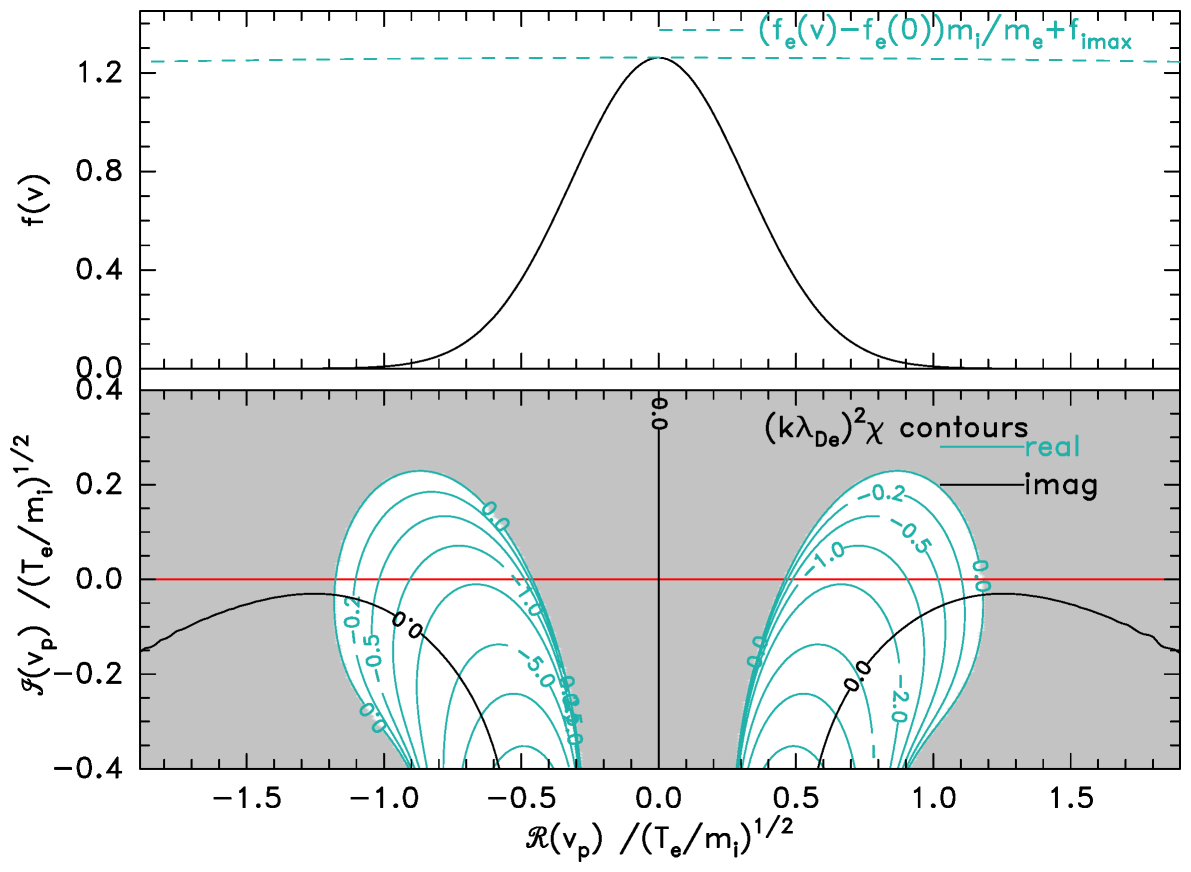
\includegraphics[width=0.7\hsize]{maxwellian}
  \caption{Contours of full susceptibility for $T_e=10$, $T_i=1$.  At
    the intersection of the black contour with the green contours, the
    wave vector $k$ is such that $k\lambda_{De}$ equals the square
    root of minus the green contour's value.}
  \label{maxwellian}
\end{figure}
The velocity units are normalized to the cold ion sound speed
$c_{s}=T_e/m_i$.  The upper panel shows the ion distribution, a simple
Maxwellian. A green dashed line is added, which shows the deviation of
the electron distribution from its peak value $(f_e(v)-f_e(0))m_i/m_e$
scaled by the mass ratio. It shows that the electron distribution
($T_e=10$ here) hardly varies across the velocity range of the ion
distribution. The lower panel plots contours of the full
susceptibility in the form $(k\lambda_{De})^2\chi$ where
$\chi=\chi_i+\chi_e$. The black contour is where the imaginary part is
zero. The green contours are labelled with values of the real
part. They are given only for negative values. In the gray shaded
region the real part is positive and no solution of the dispersion
relation exists.  Since the dispersion relation is $\chi=-1$, the
solution for a particular value of $k\lambda_{De}$ occurs at the
intersection of the black contour with the green contour corresponding
to a value $\Re(k^2\lambda_{De}^2\chi)=-(k\lambda_{De})^2$.  All such
intersections in this case are below the real axis of $v_p$, showing
that $\omega/k$ has negative imaginary part and the waves are damped
($k$ is real and $\omega$ has a negative imaginary part) in this
case. We shall later encounter unstable cases where the black contour
rises above the real $v_p$ axis in the unshaded region.

This display
thus provides graphically the entire dispersion relation for all real
$k$, in particular the zero green contour is the long-wavelength
($k\to 0$) limit.
\begin{figure}[htp]
  \centering
  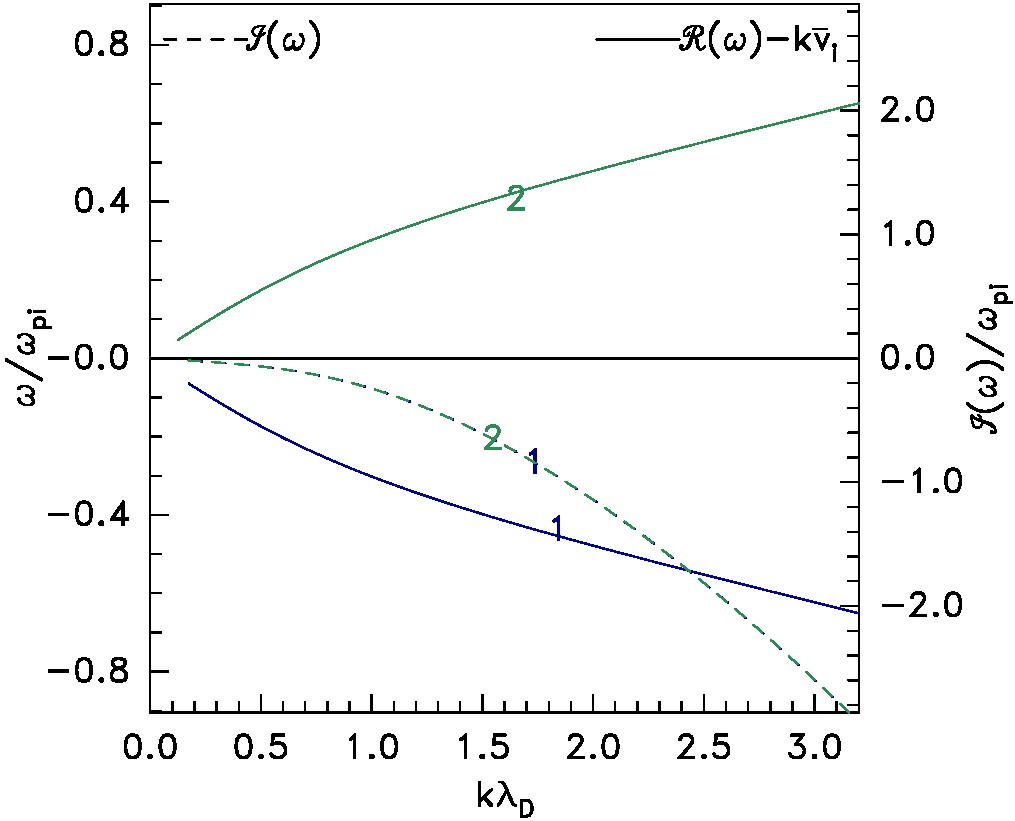
\includegraphics[width=.5\hsize]{maxwelok}
  \caption{Dispersion plot of $\omega$ versus $k$ for simple
    Maxwellian, $T_e=10 T_i$.}
  \label{fig:maxwelok}
\end{figure}
The contouring routine follows the black ($\Im(\chi)=0$) contour, and
as it does so, traces out values from small $k$,
($\Re(k^2\lambda_{De}^2\chi)\to 0$) to large $k$,
($\Re(k^2\lambda_{De}^2\chi)\to-\infty$). By collecting those values,
and recognizing that
$\omega=v_pk=v_p\sqrt{-\Re(k^2\lambda_{De}^2\chi)}/\lambda_{De}$, one
can readily construct the corresponding dispersion relation and plot
$\Re(\omega)$ and $\Im(\omega)$ as a function of $k$. Fig.\
\ref{fig:maxwelok} shows the result corresponding to Fig.\
\ref{maxwellian}. There are two branches corresponding to negative and
positive phase velocity and $\Re(\omega)$ ($k$ is taken positive). By
symmetry they both have exactly the same damping factor $-\Im(\omega)$
which makes the two dashed lines plot exactly over one another.

\subsection{Alternative Two-Tone Plot Approximation}
An alternative way to display an approximation for a range of electron
temperatures not necessarily equal to $T_0$ is the following.  We
recognize that when the phase velocity $v_p$ (relative to the center
of the electron Maxwellian) is small, the electron susceptibility in
the dispersion relation can be approximated as
\begin{equation}
  \label{dispersion}
   k^2\lambda_D^2(\chi_i+1) = - k^2\lambda_D^2\chi_e
\approx - {T_0\over T_e}\left(1+i \sqrt{\pi m_e\over
    2 T_e}v_p\right).
\end{equation}
The imaginary term in $\chi_e$ (electron Landau
damping) is smaller by the square root of the inverse mass ratio, and
significant mostly at high phase velocity. Neglecting it has the
effect of raising the black contour (on which the imaginary part of
$\chi$ is zero) toward zero at large $|v_p|$, but it has little effect
where $f_i$ is non-negligible. The real part of the dispersion
relation is simply 
\begin{equation}
  \label{ksquared}
  k^2\lambda_D^2 = -\Re(k^2\lambda_D^2\chi_i )-T_0/T_e.
\end{equation}
If $k$ is regarded as a free choice, the dispersion relation can be
satisfied at any complex phase velocity at which the right hand side
of (\ref{ksquared}) is positive: $\Re(k^2\lambda_D^2\chi_i)$ is more
negative than $T_0/T_e$, and simultaneously
$0=\Im(k^2\lambda_D^2\chi)\simeq\Im(k^2\lambda_D^2\chi_i )$. The value
of $k^2$ is given by eq.\ (\ref{ksquared}) for a root on a contour of
known $\Re(k^2\lambda_D\chi_i)$ and $T_0/T_e$.  Consequently, contours
in the complex $v_p$ plane of $\Re(k^2\lambda_D\chi_i)$ (which we've
shown depends only on the shape of the ion distribution) correspond to
contours of $k^2\lambda_D^2$, if $T_0/T_e$ is fixed. But alternatively
we can consider a range of different possible $T_0/T_e$ values, and
regard the region of existence of solutions as being bounded by
contours at which $\Re(k^2\lambda_D^2\chi_i)<-T_0/T_e$. Taking
$T_e\to \infty$ gives the largest extent
($\Re(k^2\lambda_D^2\chi_i)<0$) for which this can be satisfied, but
for any other temperature ratio the contour equal to $-T_0/T_e$ bounds
the existence region. For example when $T_0/T_e=1$, $\Re(k^2\lambda_D^2\chi_i)<-1$.

Fig \ref{maxwellion} shows what is obtained for the same
simple Maxwellian as before, choosing $T_0=10T_i$.
\begin{figure}[ht]
  \center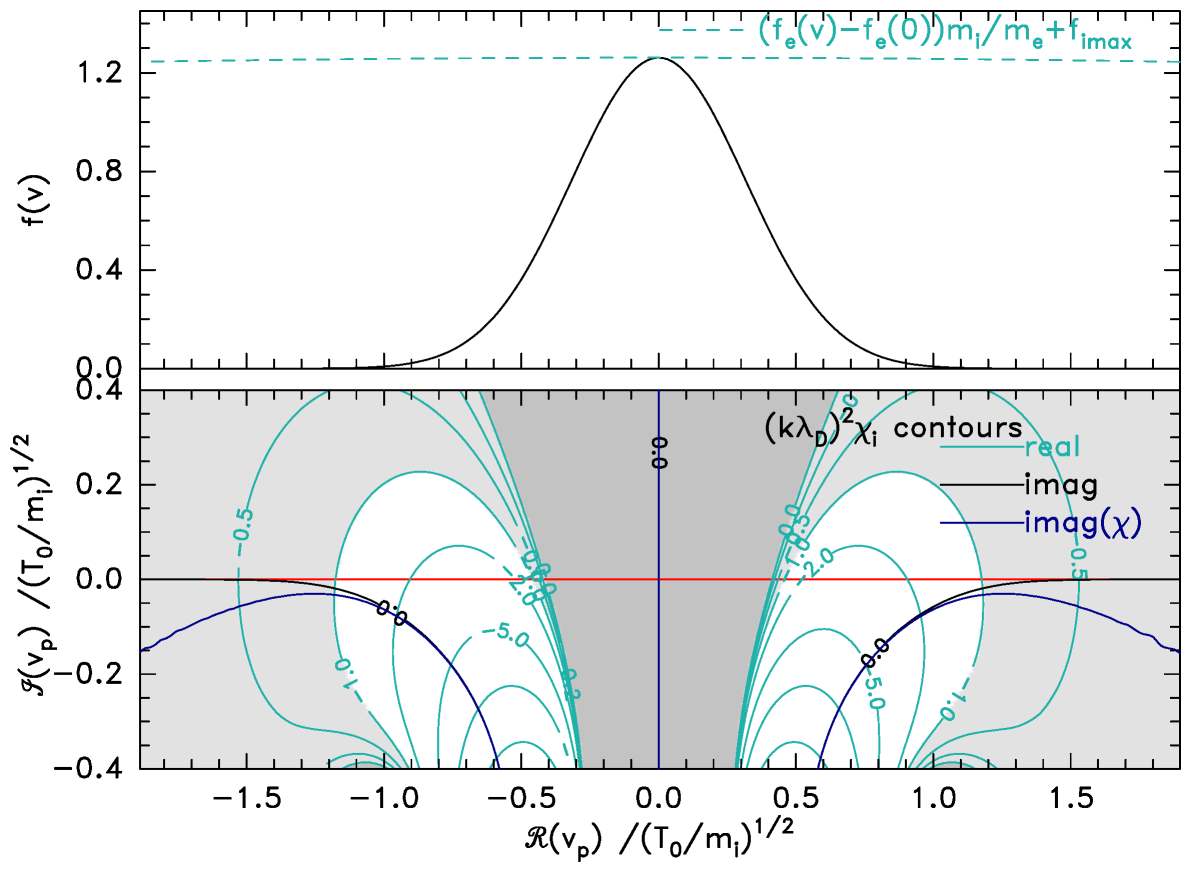
\includegraphics[width=0.7\hsize]{maxwellion}\endcenter
  \caption{Contour Plot of ion susceptibility from which the
    dispersion relation can be read. The real-part contour heights are
    logarithmically spaced, being at minus $0.,.2,.5,1.,2.,5.,10.$
    etc. These values can be interpreted as the $T_0/T_e$ at which
    each contour is the $k\to 0$ boundary of solution existence.
    Simple Maxwellian ion distribution with
    $T_0=10T_i$.\label{maxwellion}}
\end{figure}
The light-gray shaded regions are those where
$\Re(k^2\lambda_D^2\chi_i)$ is more positive than $-1$. Those are
regions where no solutions exist for $T_e=T_0$. For that electron
temperature, the dispersion relation solutions lie (only) along those
segments of the imaginary-part zero-contour that lie in unshaded
regions. Those unshaded regions are actually identical to the unshaded
regions of Fig.\ \ref{maxwellian}, in so far as the approximation 
$\Re(k^2\lambda_{De}^2\chi_e)=T_0/T_e$ holds. The real contour values differ
from those in Fig.\ \ref{maxwellian} by $-1$. Although the green and black
contours are of $\chi_i$, the actual dispersion relation requires
$\Im(\chi)=0$, using the full $\chi=\chi_i+\chi_e$. By plotting in
addition the zero contour of $\Im(\chi)$ (for the case $T_e=T_0$): the
blue line, one obtains the full solution (following the blue line and
finding its intersections with the green) of the dispersion for that
case. The black line is the $\Im(\chi)=0$ contour ignoring electron
Landau damping, which is exact only when $T_e\to\infty$. So the
difference between the black and blue contours indicates the degree of
approximation involved in ignoring electron Landau damping for
$T_0/T_e=1$. At any electron temperature between $T_0$ and $\infty$
the corresponding imaginary contour would lie between the blue and the
black curves.  At any point along such curves, the real part of
$k^2\lambda_{D}^2 \chi_i$ can be read from the green contours that
intersect it. Knowing $k^2\lambda_{D}^2 \chi_i$ one can immediately
deduce the value of $k$ from eq.\ (\ref{ksquared}).
 The edge of the allowed
solution region for a $T_e$ different from $T_0$ is at the contour
where $\Re (k^2\lambda_{D}^2 \chi_i)=-T_0/T_e$. So the green contours
can be considered universal for any $T_e$. For example, if
$T_e=20T_i=2T_0$, then the $-0.5$ contour is the allowed solution
boundary.

Omission of electron Landau damping hardly affects the black contour
in the unshaded region, but it raises it toward $v_{pi}=0$ further out
in the light shaded region. The smallest $k$ solution for $T_e=T_0$ :
the long wavelength solution, occurs at the boundary with the (light)
shaded region where $\Re (k^2\lambda_{D}^2 \chi)= 0$ and
$\Re (k^2\lambda_{D}^2 \chi_i)= -1$.  In Fig \ref{maxwellion}, that
position is at $\Re (v_p)\approx\pm 1.15 c_{s}$ because $T_i/T_0=0.1$
in this case, and the actual warm-ion acoustic speed for such waves is
approximately $\sqrt{(T_e+3T_i)/m_i}$. If instead $T_e=2T_0$, the long
wavelength root (contour $-0.5$) has $v_p$ just over $1.5$. Or again,
if $T_e=0.5T_0$ the solution boundary is at the $-2.0$ contour.  The
imaginary part of $v_p$ is everywhere negative along the solution
curve (blue) in this plot, indicating that these waves are damped. The
damping rapidly becomes stronger as one moves away from the shaded
edge because the real part becomes large (and negative) implying large
$k$, and thus large $\omega_i$ (because $\omega_i =kv_{pi}$).

An important caveat for the alternative two-tone treatment is that the
approximations employed are appropriate only for small phase velocity
relative to electron thermal velocity. When $v_p/c_s\gtrsim
\sqrt{m_i/m_e}/5$ it should not be used. 

\section{One-dimensional Examples}
\subsection{Current-driven Instabilities}

When both electrons and ions are Maxwellian but their central
velocities differ, a current is present. Ignoring the fact that it
will perturb the magnetic field, we can still examine electrostatic
stability. We choose to express velocities relative to the mean
electron velocity, but still in units of the ion acoustic speed. 

\begin{figure}[htp]
\center
  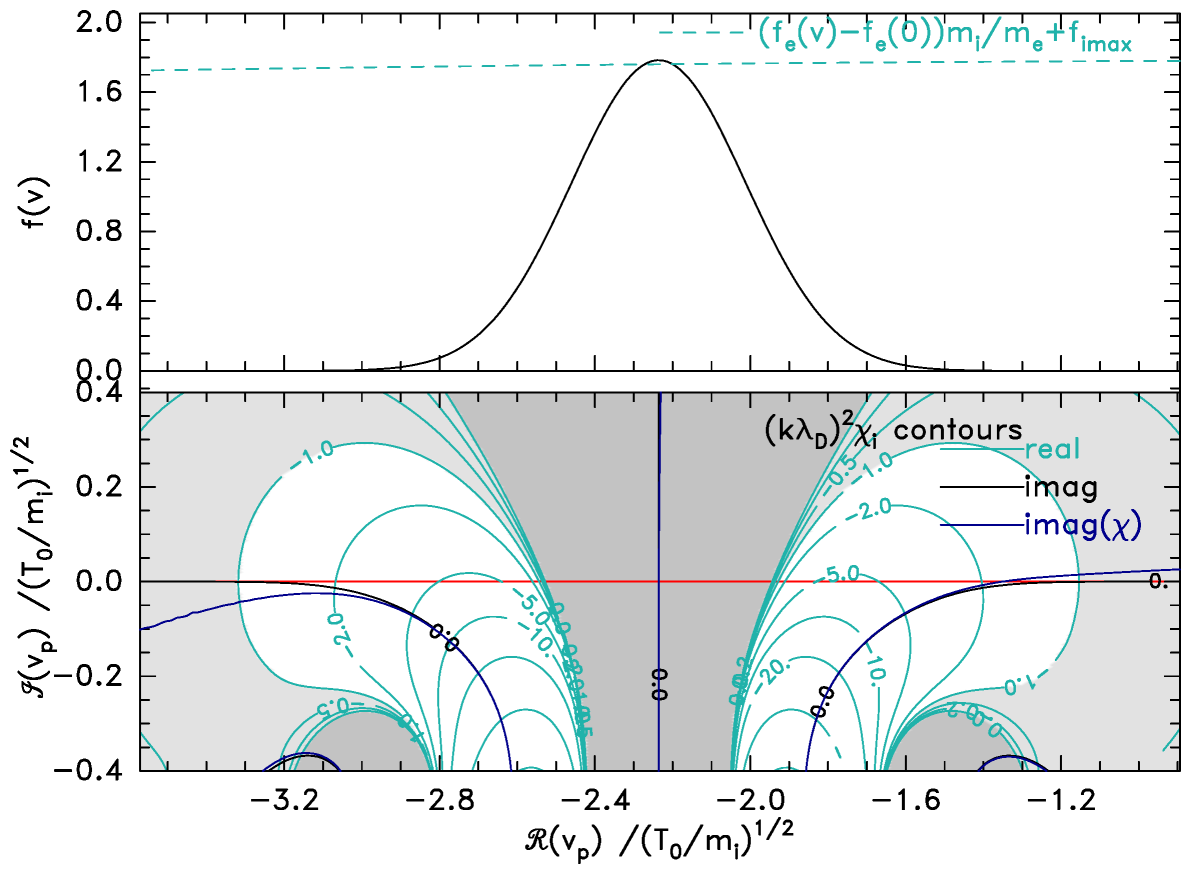
\includegraphics[width=0.48\hsize]{ionacoustic1}\hskip-1em(a) 
  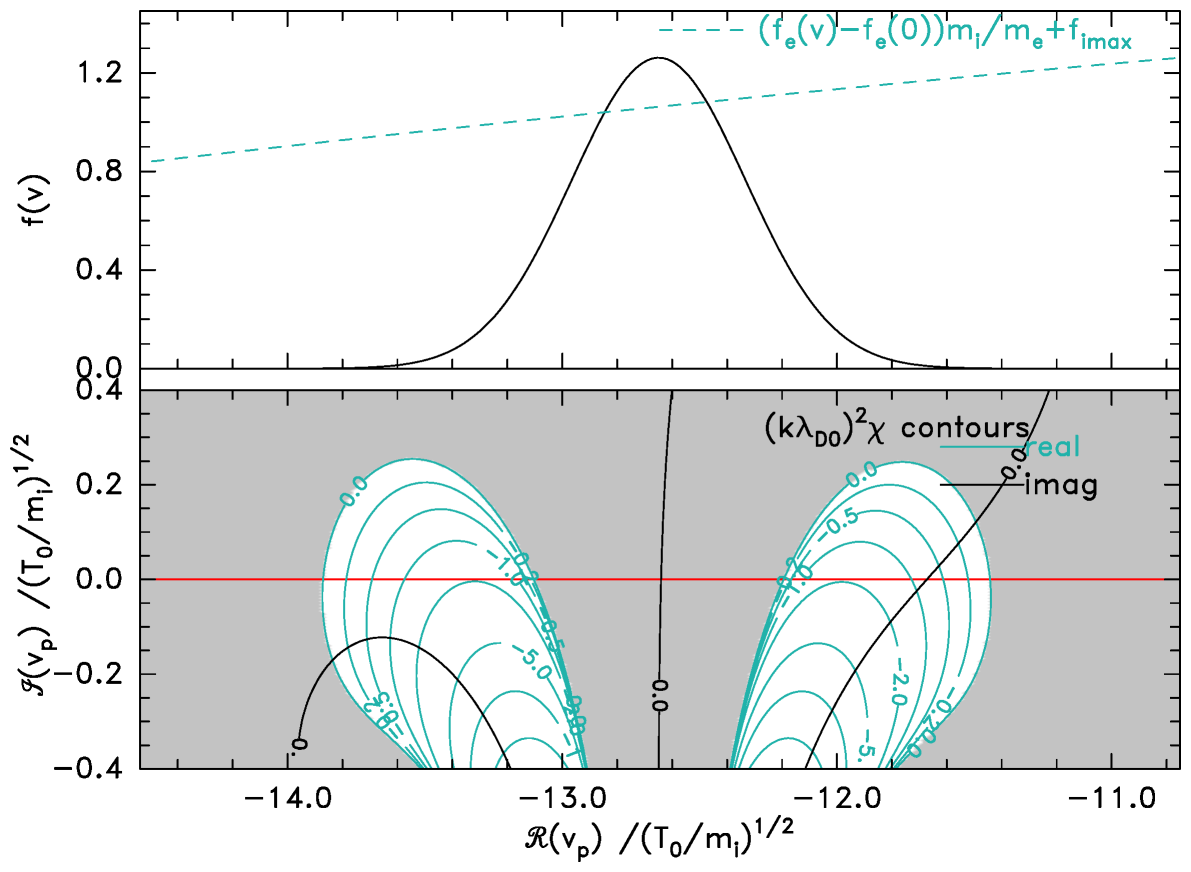
\includegraphics[width=0.48\hsize]{ionacoustic2}\hskip-1em(b)
  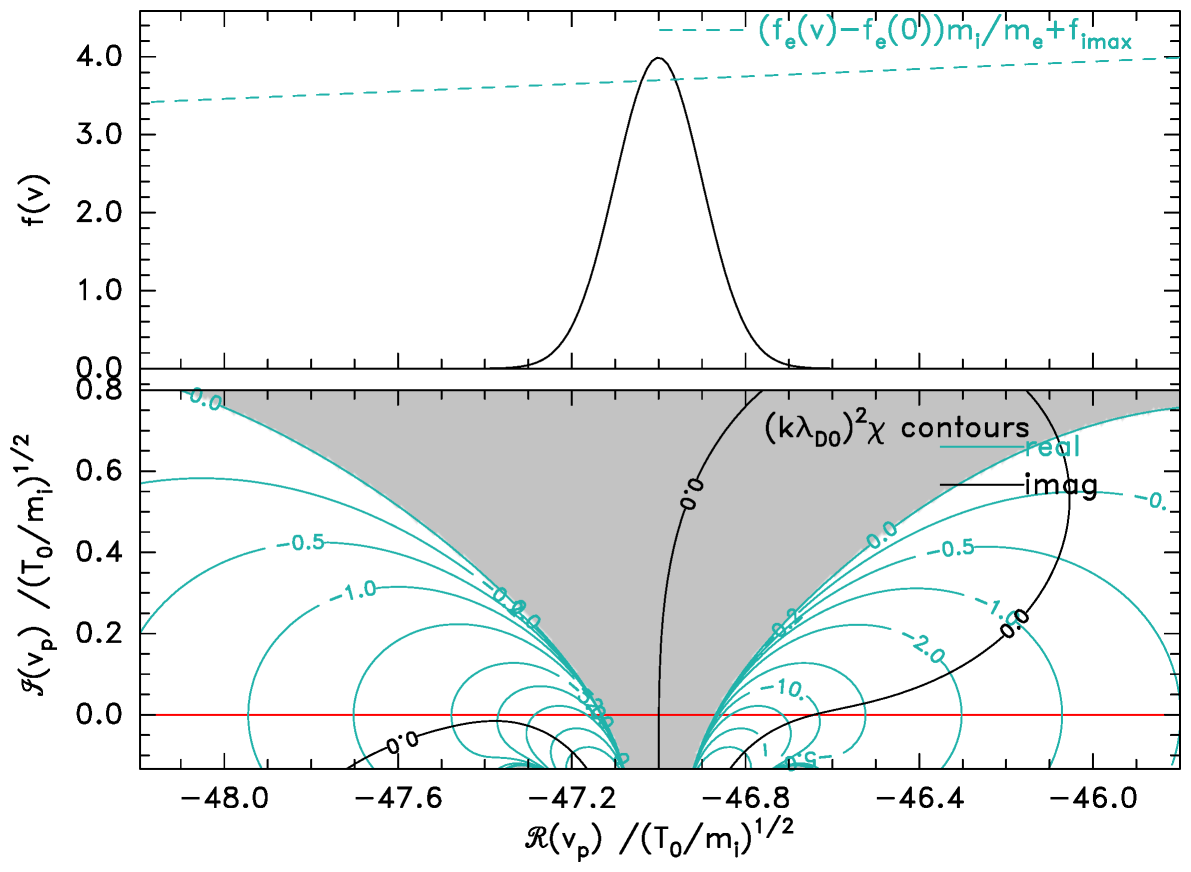
\includegraphics[width=0.48\hsize]{ionacoustic3}\hskip-1em(c)
  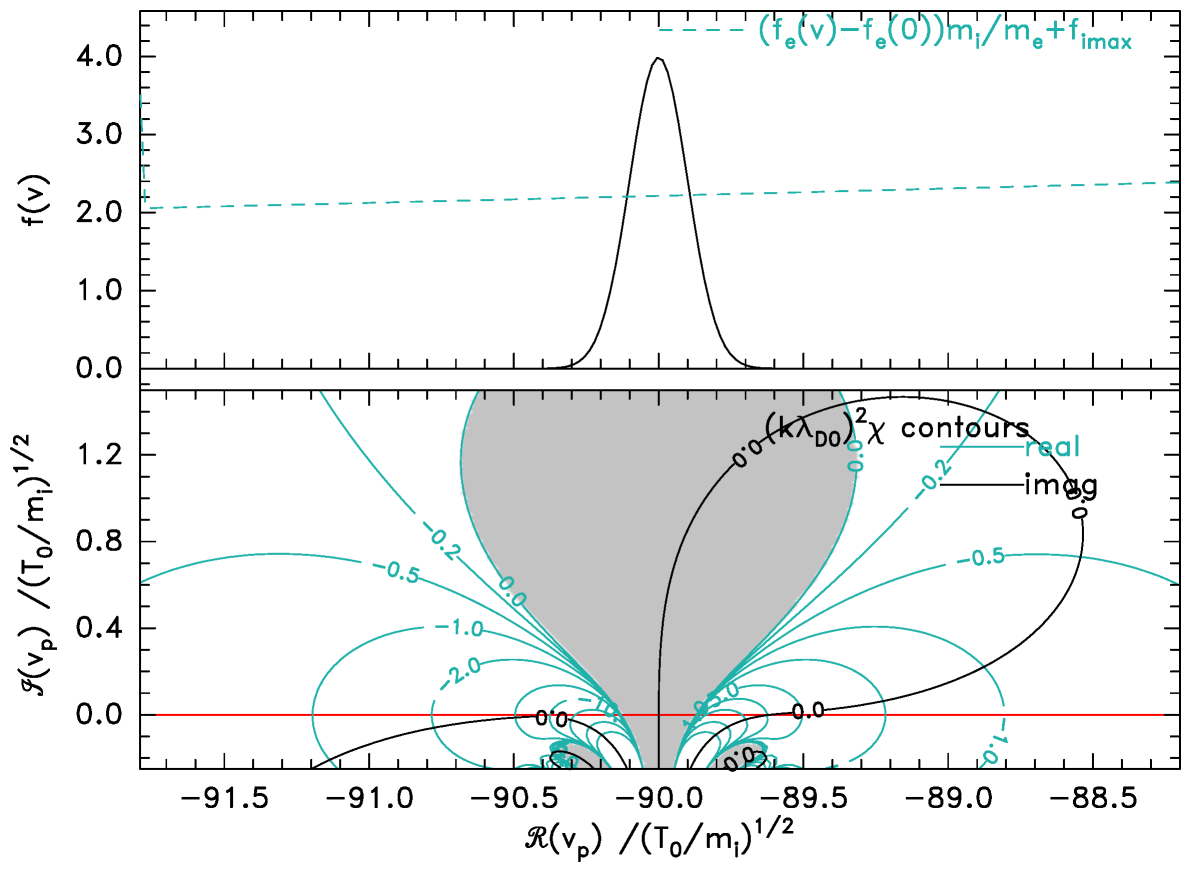
\includegraphics[width=0.48\hsize]{ionacoustic4}\hskip-1em(d)
  \caption{Ion acoustic instability for $T_i=1$, (a) $T_0=20$,
    $v_i=-10\sqrt{T_i/m_i}$, (b) $T_0=10$, $v_i=-40\sqrt{T_i/m_i}$ (c)
    $T_0=100$, $v_i=-470\sqrt{T_i/m_i}$ (d) $T_0=100$,
    $v_i=-900\sqrt{T_i/m_i}$. In (b)-(d) the unapproximated electron
    susceptibility is used; and $f_e$ scaled to the same height as
    $f_i$ is plotted, showing the very slight positive $df_d/dv)$ and
    how far out on the electron Maxwellian the plot is. Cases (c) and (d)
    are effectively Buneman instabilities accounting for finite ion
    temperature.  
    \label{ionacoustic1}}
\end{figure}
\paragraph{Ion acoustic instability} can be driven by current that
corresponds to quite moderate ion velocity shift when the temperature
ratio $T_e/T_i$ is high enough. Fig.\ \ref{ionacoustic1}(a)
illustrates a case with a moderate ion velocity shift
$-10\sqrt{T_i/m_i}=-2.24\sqrt{T_e/m_i}$. The ratio $T_e/T_i=20$ makes
ion Landau damping negligible and the black lines (omitting the
imaginary $\chi_e$) are extremely close to the real axis away from the
ion distribution region. But including $\Im(\chi_e)$ the positive
slope of the electron distribution causes the blue line to rise above
the real axis on the right of the ions: unstable growth. This is the
current-driven ion acoustic instability. On the left damping occurs.
Fig.\ \ref{ionacoustic1}(b) shows a much greater
velocity shift, having larger $\Im(v_p)$ even with lower
$T_e=T_0=10T_i$, but it is a qualitatively similar ion-acoustic wave. 
Fig.\ \ref{ionacoustic1}(c) and (d), having $T_e=100T_i$ would be
reasonably represented by a fluid ion treatment, and in fact
correspond to \textbf{Buneman instabilities}. Buneman's original treatment
used cold fluid ions. 

\begin{figure}
  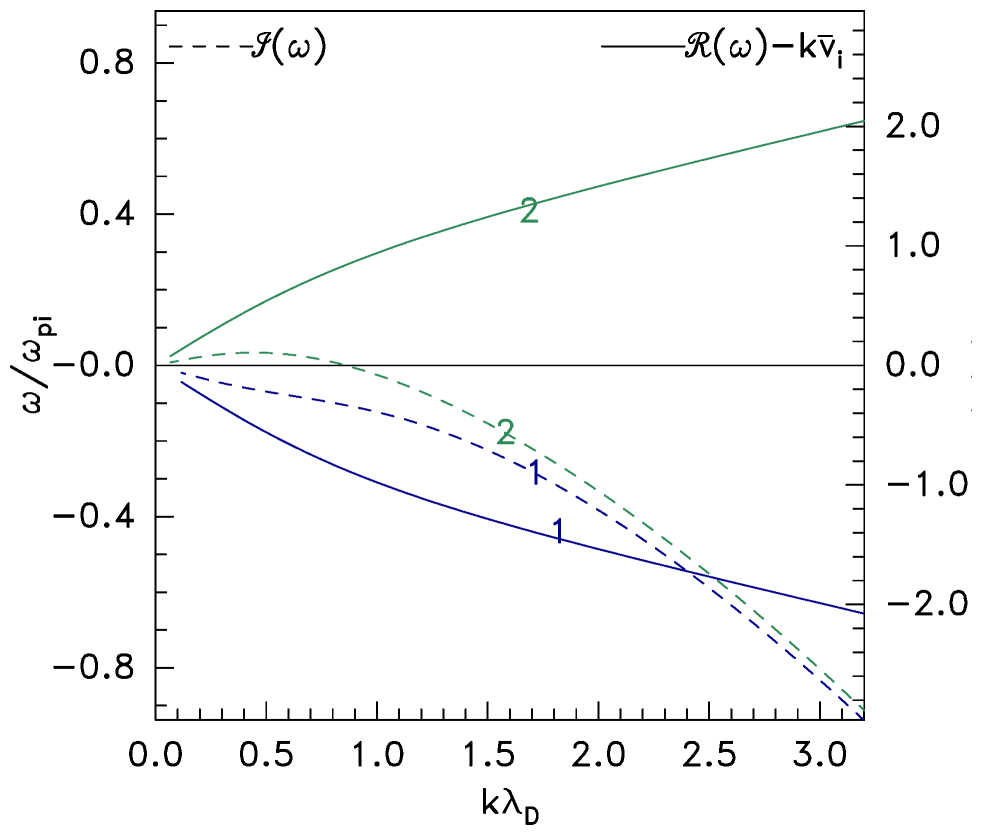
\includegraphics[width=0.48\hsize]{ovk2}\hskip-1em(a)
  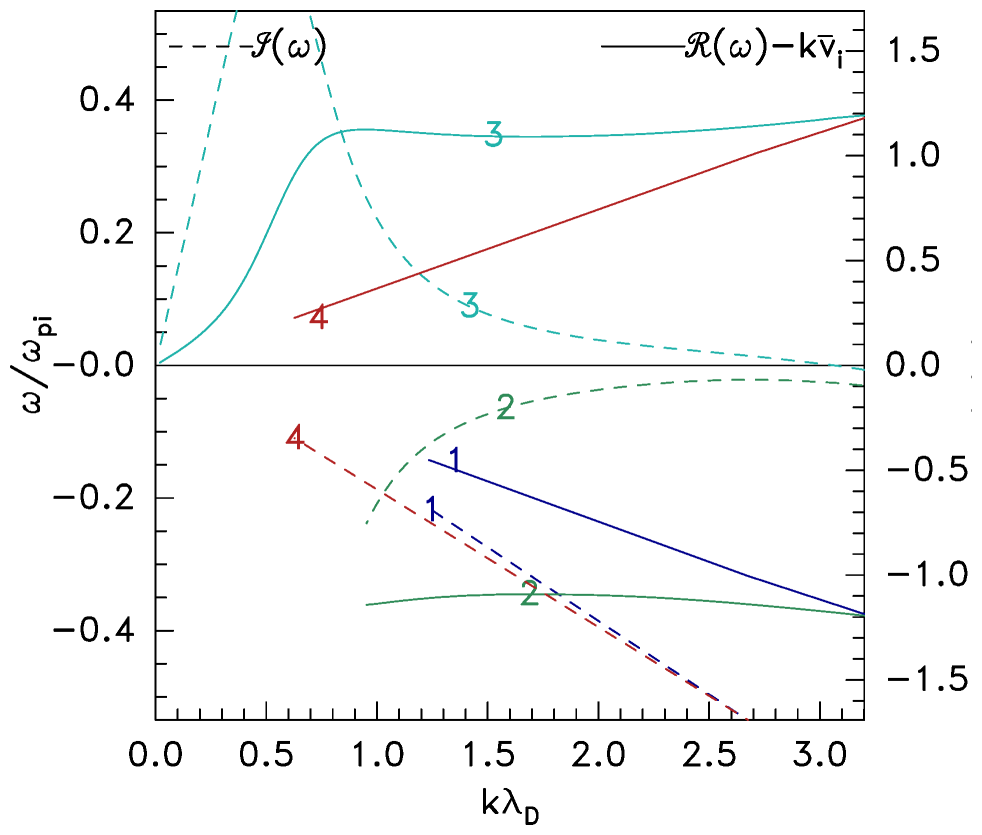
\includegraphics[width=0.48\hsize]{ovk4}\hskip-1em(b) 
  \caption{Dispersion curves (a) corresponding to Fig
    \ref{ionacoustic1}(b) and (b) corresponding to Fig
    \ref{ionacoustic1}(d). The real frequencies (solid lines)
    displayed are in the frame of reference of the mean ion velocity
    ($\Re(\omega)-k\bar v_i$). The curves labelled 2 are the unstable
    roots with dashed (imaginary) curves rising above
    zero.\label{ovk}}
\end{figure}

The main point of this comparison is to show that there is no
qualitative distinction between ion-acoustic instability and Buneman
instability. From the viewpoint of a Penrose analysis they both arise
from the formation of a local minimum in the combined distribution
$f_e+(m_e/m_i)f_i$. Or in other words from a positive slope of $f_e$
at phase speeds where the real part of $\chi$ is negative, permitting
a solution of the dispersion relation (with real $k$). As the velocity
shift magnitude increases, ion acoustic and Buneman instabilities
connect continuously.

Fig.\ \ref{ovk} shows conventional dispersion curves of $\omega$
versus $k$, expressed in the ion frame, for two of the cases of Fig.\
\ref{ionacoustic1}. The large-shift Buneman regime (b) has faster
instability peak growth rate by a factor of approximately 20.


\subsection{Positive-slope $f_i$ tail}
A different sort of ion distribution is shown in Fig \ref{flattail}, where a relatively
\begin{figure}[ht]
  \center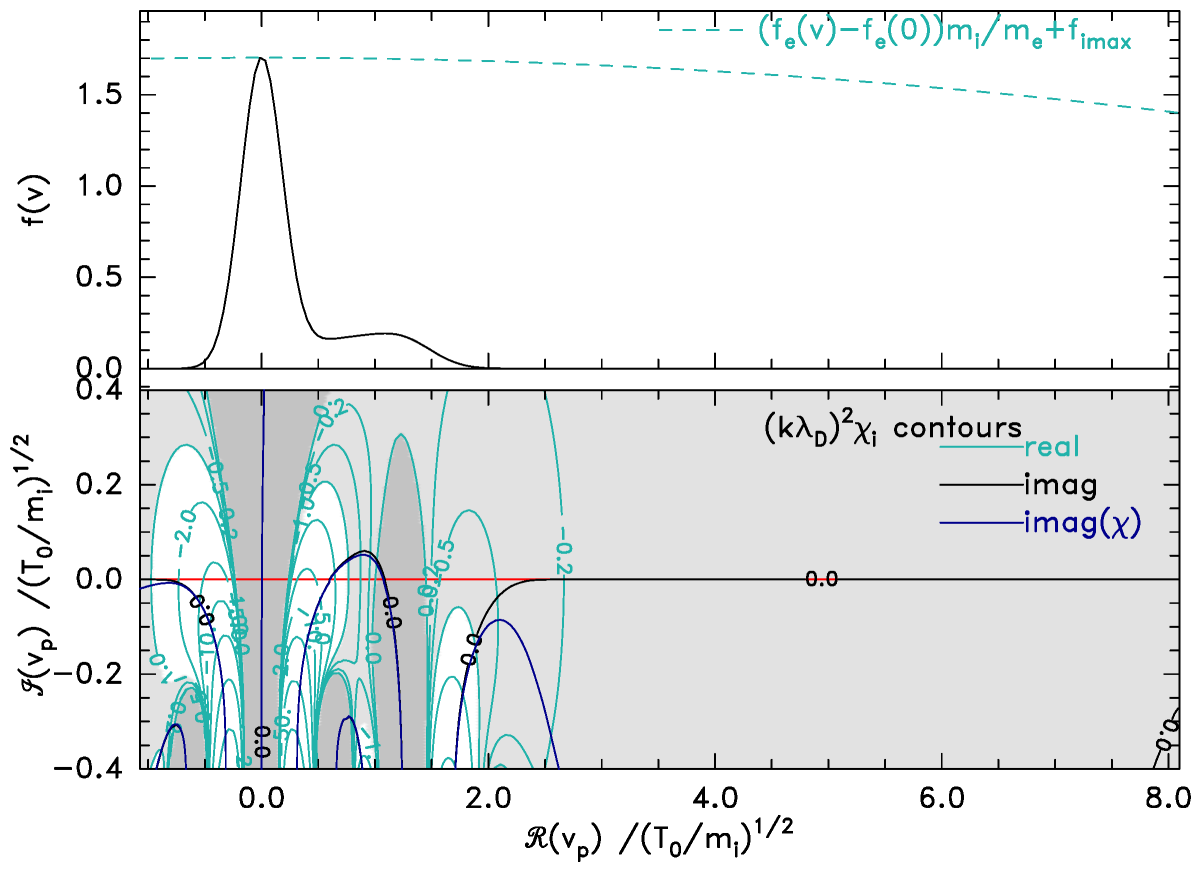
\includegraphics[width=0.8\hsize]{flattailion}\endcenter
  \caption{Contour Plot of ion susceptibility for an ion distribution with
    a long tail of slightly positive slope, showing unstable
    regions. $T_0=30T_i$. \label{flattail}}
\end{figure}
long tail of slightly positive slope is added to the Maxwellian bulk
(whose temperature is $T_0/30$). The tail induces an ion-acoustic
instability (sometimes called ``ion-ion'' but not entirely
appropriately in this case), but requires no current (i.e.\ electron
shift) to do so. The instability is in the region where the
$\Im(\chi_i)=0$ contour rises above the real $v_p$-axis, corresponding
to wave growth. The unstable solutions actually exist only near the
low-velocity end of the tail for $T_e=T_0$. In the higher-velocity
range, although the contour is still at positive $v_{pi}$ it is in the
light shaded $v_p$ region where the real part of $\chi$ is positive
and the dispersion relation cannot be satisfied. This observation is
an important corrective to any improper transference of intuition
derived from \emph{electron} stability of Langmuir waves. Unstable
Langmuir waves exist on an electron-distribution-tail throughout most
of the region where its slope is positive. That is not the case for
ion-acoustic instability.

Actually a direct quantitative understanding of this difference can be
derived from the figure. In the limit $T_e\to \infty$, the electrons
contribute negligibly to the total susceptibility. Only the ion
contribution need be considered. In that case the dispersion relation
(along the black line) is \emph{exactly} the same as it would be for
Langmuir waves of electrons of the same distribution (scaling the
velocities appropriately, see section \ref{elecLang}). We see that
then the solution region (outside the dark grey shading) extends
almost (but actually not quite) to the upper end of the positive slope
region. This is exactly the region of Langmuir wave instability for an
electron distribution of this shape. So there is a precise analogy
between the ion and electron distribution positive-slope Landau growth
at $T_e\to\infty$. However, as $T_e$ is lowered, the electron
contribution to $\chi$ becomes significant, and causes the solution
region to contract towards the lower velocity end of the tail. If
$T_e$ becomes less than approximately $T_0/3$, the solution region
(whose boundary is then on the $\sim-3$ contour) no longer contains
any positive-$\Im(v_p)$ regions of the $\Im(\chi_i)=0$ contour. The
ion instability disappears.  The last phase velocity to remain
unstable is where the $\Im(\chi)=0$ contour crosses the x-axis:
$v_p\approx 0.5 c_s$. This suppression of ion-ion instability by
lowering of $T_e$ is \emph{nothing to do with electron Landau
  damping}, which is still negligible, as evidenced by the equality of
the black and blue curves in this vicinity. It is caused by the real
part (not the imaginary part) of the electron susceptibility.

In the opposite direction to the tail, a relatively weakly damped
acoustic branch exists. A third branch, which is strongly damped
unless $T_e$ is very high, exists just beyond $2c_{s}$, and some other
extremely heavily damped branches of little practical relevance also exist at
$\Im(v_{p})<-0.3$. Those heavily damped branches are omitted from the
$\omega(k)$ dispersion plot of Fig.\ \ref{fig:flattailok}.
\begin{figure}[htp]
  \centering
  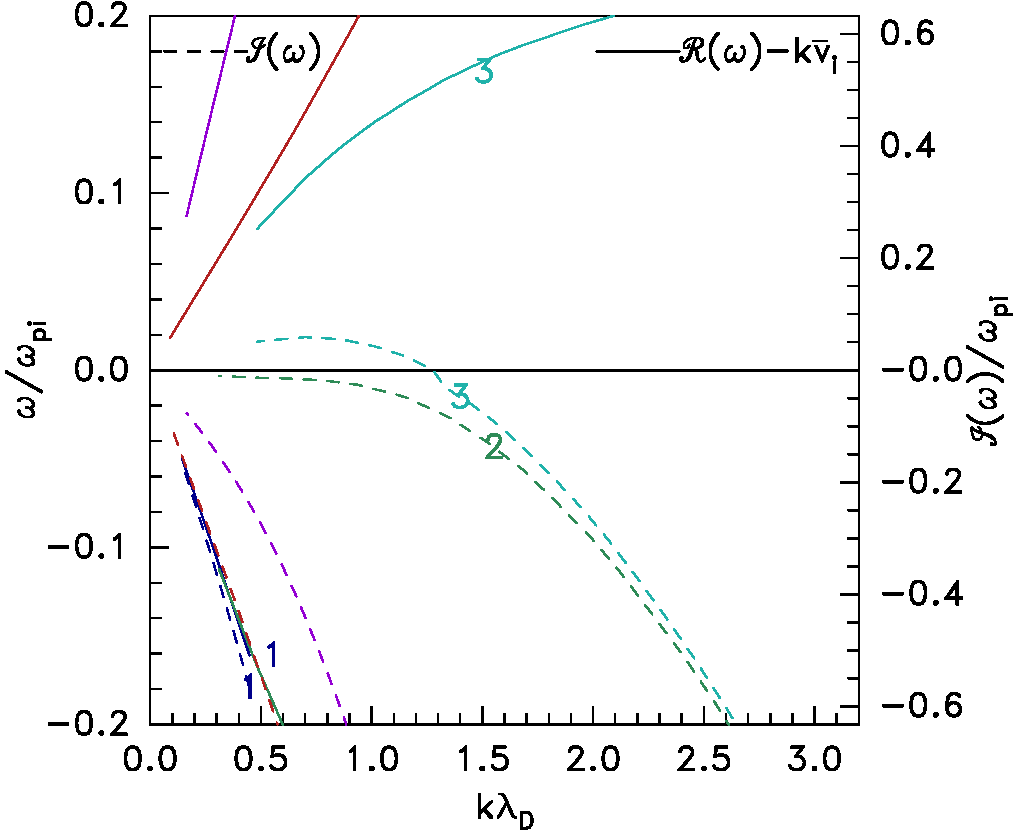
\includegraphics[width=0.5\hsize]{flattailok}
  \caption{Dispersion curves for the $T_e=T_0=30T_i$ case of Fig.\
    \ref{flattail}.}
  \label{fig:flattailok}
\end{figure}
The branch 2 is now unstable for $k\lambda_D\lesssim 1.4$.

\subsection{Two shifted ion populations}
\begin{figure}[htp]
  \center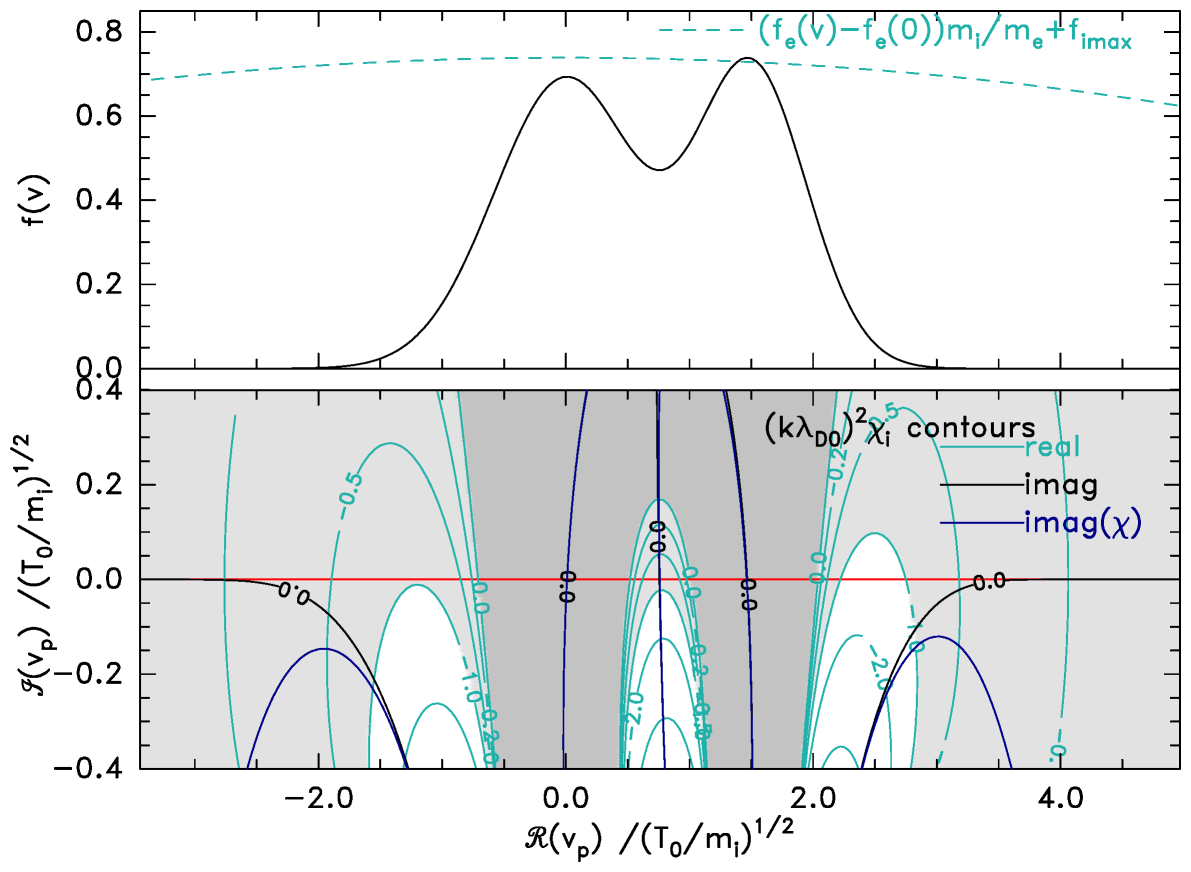
\includegraphics[width=.7\hsize]{twogaussLowTe}\endcenter
  \caption{Contour Plot of ion susceptibility for an ion distribution
    with two humps. $T_0$ is 3 times the temperature of the unshifted
    hump. It can be called an ion-ion or ion-two-stream instability.\label{twogausslowTe}}
\end{figure}
Fig.\ \ref{twogausslowTe} shows an ion distribution with two
overlapping humps.  The reference temperature is taken as 3 times the
temperature of the unshifted hump (the other hump has width
corresponding to a temperature 0.6 times lower). When $T_e=T_0$, waves
are only just unstable in the distribution minimum near
$v_p=1.2$. Lower $T_e$ would not be unstable. Higher $T_e$ permits
greater growth rate, again indicating the importance of $T_e$ in
determining stability, but again not arising from electron Landau
damping. For five times higher $T_e$ the maximum growth rate of the
instability is greatly increased, yet the range of real part of the
phase velocities that are unstable is extremely narrow, residing at
the bottom of the valley between the humps, where electron Landau
damping is unimportant. This near-vertical branch of the imaginary
zero-contour is completely separate from the ion-acoustic branches at
left and right, which in this case are strongly Landau damped. The
instability is therefore clearly not ion-acoustic, and could be called
``ion-ion'', or perhaps ``ion-two-stream''. 


Fig.\ \ref{separatehumps} shows a case by contrast in which two
Gaussian humps have negligible overlap.
The stable ion sound branches for the two humps are clearly visible.
The centers of the ion humps are separated by just over twice
$c_s$. The result is that the allowed solution regions (unshaded) for
$T_e=T_0$ merge in the middle, producing an unstable region along a
section of the vertical $\Im(\chi)=0$ branch. Lower temperatures
(e.g. the -2.0 contour, $T_e=0.5T_0$) don't merge and so do not have
unstable solutions, higher temperatures (light gray) have greater
extent and growth rate of instability.
\begin{figure}[htp]
  \center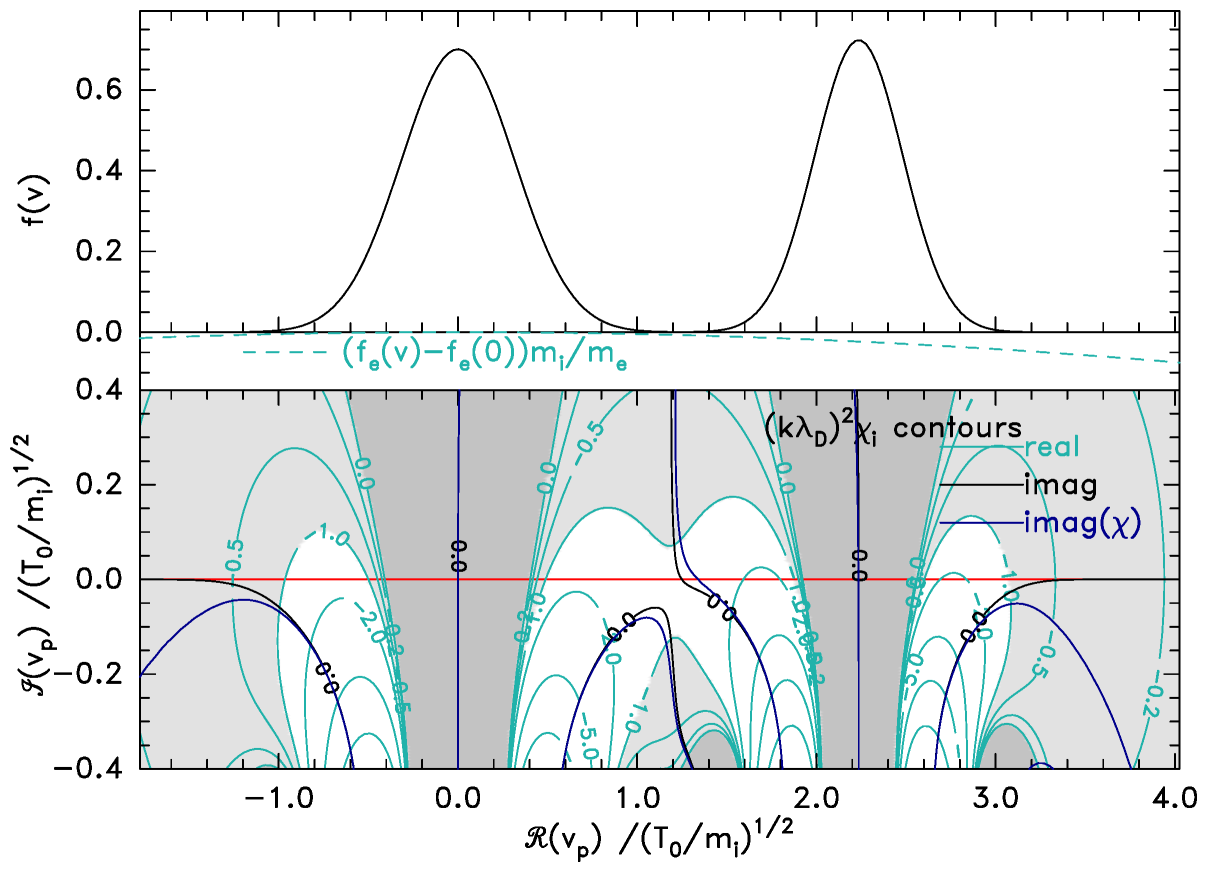
\includegraphics[width=0.7\hsize]{twonarrowgauss}\endcenter
  \caption{Contour Plot of ion susceptibility for an ion distribution
    with two well separated Gaussians. $T_0$ is 10 times the
    temperatures of the centered ion Gaussian. \label{separatehumps}}
\end{figure}
Generally speaking, humps separated by more than twice the ion sound speed
don't lead to instability. Stringer\footnote{T E Stringer, Plasma
  Physics, {\bf 6}, 267-279 (1964).} gives a criterion $1.3 v_{ti}<
\Delta v/2 < \sqrt{T_e/m_i}$ for ion-ion instability when equal
Maxwellian ion distributions are separated by velocity $\Delta v$.

\section{Oblique Propagation}

So far the analysis has been of electrostatic waves either in an
unmagnetized plasma or propagating parallel to the magnetic field.
Moreover here and in subsequent analyses the distribution function to
be used has been the one dimensional distribution, i.e.\ integrated
over velocities perpendicular to the wavevector $\bm k$. In this
section multidimensional effects are discussed arising from oblique
propagation with $\bm k$ not parallel to $\bm B$.

\subsection{Beam-like Ion distributions in 3-D}
If the ion distribution in three velocity directions were really
represented by two shifted but otherwise isotropic finite width beams
(e.g.\ shifted 3-D Gaussians) and the plasma were unmagnetized, then
the relevant velocity shift between the beams as viewed in the
one-dimensional distribution is equal to the velocity shift in 3-D,
$|\bm{\Delta v}|$, times the cosine of the angle between $\bm k$ and
the direction of velocity shift i.e.\
$\bm k.\bm{\Delta v}/(k\Delta v)$. If then $\Delta v$ is large enough
in one dimension to avoid ion-ion instability because
$\Delta v \gtrsim 2\sqrt{T_e/m_i}$, that does \emph{not} make an unmagnetized
plasma stable. Instead we would require
$\bm{k.\Delta v}/k \gtrsim 2\sqrt{T_e/m_i}$ for \emph{all possible
  propagation directions}. Clearly that can never be satisfied,
because we can make the wave vector and shift directions as near to
perpendicular as we like. 

In general then, unmagnetized plasmas with two widely spaced ion beams
are hardly ever completely stabilized against ion-ion instability,
because along some angle of propagation relative to the spacing, they are
not widely spaced. (However, a spherically symmetric hollow distribution could
be stable.)

The most common magnetized situation for oblique propagation of ion
waves is that the electron cyclotron frequency is much higher than
that of the waves, while the ion cyclotron frequency is much
lower. Thus to a first approximation electrons are strongly
magnetized, moving only parallel to the magnetic field, while ions are
unmagnetized. Since complete magnetization of electrons changes their
susceptibility only by replacing $v,\ v_p$ in the integral by
$v_\parallel,\ v_{p\parallel}$, or equivalently making the argument of
eq.\ \ref{chiefull} $x=\omega/k_\parallel \sqrt{2T_e/m_e}$, oblique
propagation relative to the magnetic field mostly narrows the
effective electron distribution, enhancing electron Landau damping (or
growth) at the low speeds typical of ion waves, for constant
$f_{ik}(v_k)$. However, as we have just seen, electron Landau damping
is a relatively unimportant effect for controlling the ion-ion
instability of separated beams. Electrons' more important influence is
in setting the height of the combined distribution function and
thereby affecting the real part of the susceptibility. That is not
changed by magnetizing the electrons at an angle to $k$.

\subsection{Oblique Electron-Ion instability}

By contrast, if a positive slope of the electron distribution in the
direction away from the mean ion velocity exists at the resonant
velocity, as it does for ion-acoustic or Buneman instabilities, giving
a local minimum in the combined distribution, the enhancement of
parallel \emph{slope} of magnetized electron distribution at oblique
propagation can lead to enhanced instability.  Oblique propagation for
magnetized electrons makes the electron contribution depend on the
angle $\theta$ between ${\bf k}$ and ${\bf B}$, because at constant
$v_{p\parallel}$, $\partial f /\partial v_k$ is proportional to
$1/\cos(\theta)=\sqrt{1+v_\perp^2/v_\parallel^2}$. Lower Hybrid waves
can then experience instability when $\cos(\theta)$ is small.
Magnetization of the electrons (but not ions response) makes the Penrose
combined distribution
$f_i(v_k)+f_{e\parallel}(v_{e\parallel})m_i/m_e=f_i(v_k)+f_{e\parallel}(v_kk/k_\parallel)m_i/m_e$. Then
the electron velocity scale of the electron contribution in Figure
\ref{fig:penrose} changes with the propagation angle
$\theta=\cos^{-1}(k_\parallel/k)$. The electron contribution becomes
narrower in $v_k$ as the corresponding $v_{e\parallel}=v_k/\cos\theta$
increases, but without changing in height. Consequently its derivative
with respect to $v_k$ increases.

The direction of the ion distribution components' shift
$\bm\Delta\bm v$ is taken as being along $\bm B$, so the same
geometrical compression factor $\cos\theta$ applies for ion velocity
shifts and electron distribution. However, Lower Hybrid waves in some
circumstances must account for an extra partially-magnetized electron
response term $\chi_{e\perp}=(\omega_{pe}/\Omega_e)^2\sin^2\theta$
added to the parallel susceptibility
$\chi_{e\parallel}$. This term $\chi_{e\perp}$ is not $\propto 1/k^2$,
so its relative influence depends on $k$ as well as $v_p$. However,
it is a positive definite real term added to $\chi_e$, so its
influence is always to reduce the (unshaded) area of the contour plot
in which $\Re(k^2\lambda_{De}\chi)<0$, no matter the value of $k$. It
does not change $\Im(k^2\lambda_{De}\chi)$ so the contour of
$\Im(k^2\lambda_{De}\chi)=0$ remains unchanged. Therefore addition of
$\chi_{e\perp}$ reduces the range of phase-velocities over which
solutions of the dispersion relation exists, and cannot itself induce
instability in an otherwise stable plasma.

\section{Electron Waves}

\subsection{Electron Langmuir Waves}
\label{elecLang}

The same display can also calculate the dispersion of electron
Langmuir waves. Consider a high-frequency situation in which $\chi_i$
can be ignored and $\chi_e$ is the electron susceptibility for an
arbitrary electron distribution function. Regard that distribution as
being given by the upper frame of the plot (what in the ion acoustic
analysis is the ion distribution function). Take the reference
velocity to be $\sqrt{T_0/m_e}$. The dispersion relation is then
$\chi_e=-1$. Since the shape of the distribution function and the complex
$v_p$ together determine the value of $k^2\lambda_D^2 \chi_e$ (eq.\
\ref{ionint}), the dispersion relation is satisfied for some real
value of $k$ at points in $v_p$ space where the value of the real part
of $k^2\lambda_D^2 \chi_e$ is negative and the value of its imaginary
part is zero, just as before.  Therefore we exchange the roles of
electrons and ions. We consider the plot to be for electron
susceptibility. The solution of the dispersion relation is where the
imaginary part is zero and the real part is negative. (Using the
special value switch \verb!-T99!, is programmed turn off extra Maxwellian
electron influence and to label the plots for electrons
rather than ions, as illustrated in Fig.\ \ref{langmuir}.)
\begin{figure}[ht]
\center
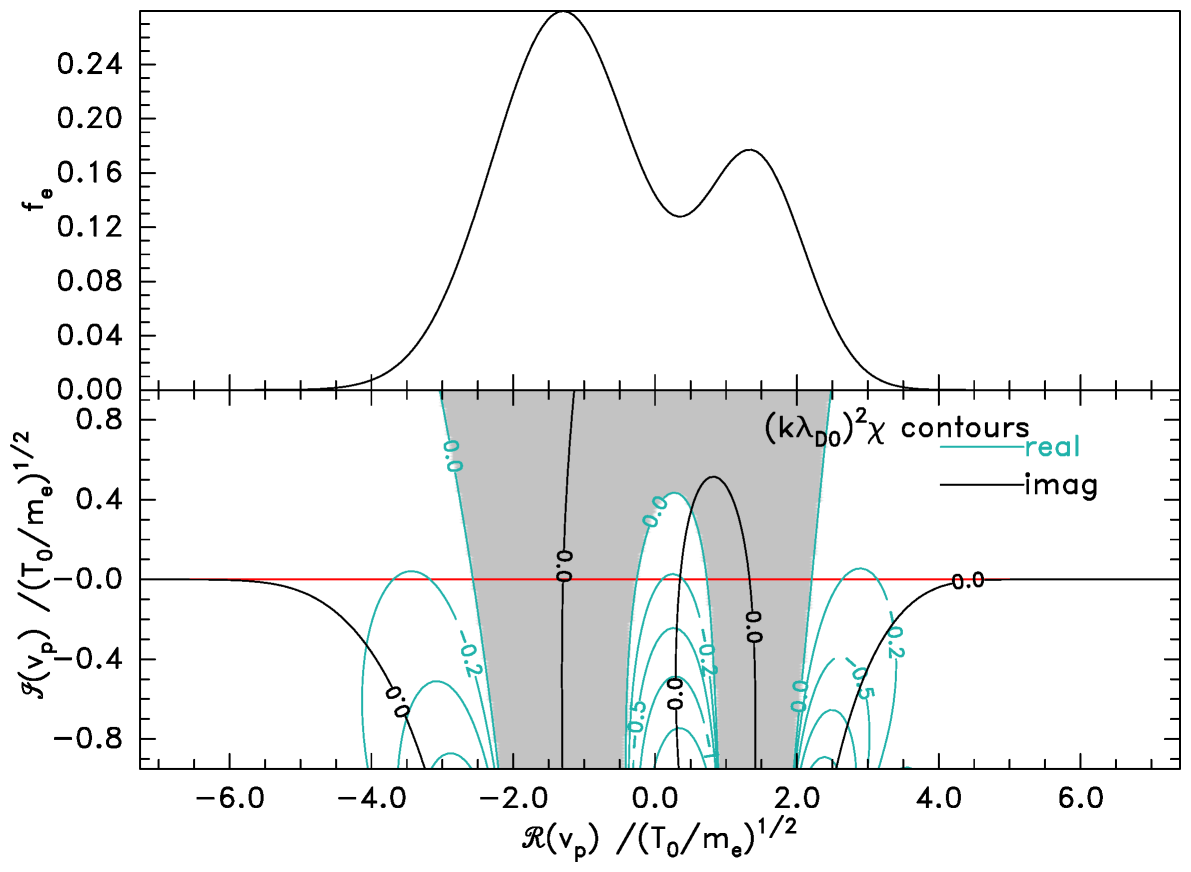
\includegraphics[width=0.7\hsize]{langmuir}
\caption{Langmuir wave pure electron case with double humped
  distribution, giving warm two-stream instability.\label{langmuir}}  
\end{figure}

This reversal of
roles helps one to understand the qualitative difference between ion
acoustic stability and Langmuir stability. It lies purely in the fact
that non-zero electron susceptibility shifts the real contours of the
ion acoustic case. When $T_e/T_0\to\infty$, and $\chi_e$ becomes
negligible, the ion acoustic instability is exactly equivalent to the
Langmuir stability with appropriately scaled velocity.


\subsection{Electron-acoustic waves}

A type of wave occurring in non-Maxwellian electron distributions with
two components of different temperatures is often called the
electron-acoustic wave. There is nothing particularly different about
such waves except that normal Langmuir waves are strongly damped
unless their phase speed substantially exceeds the electron thermal
speed. That criterion, $\omega/k\gg \sqrt{T_e/m_e}$, is equivalent to
$k\lambda_{De}\ll 1$, taking $\omega\simeq \omega_{pe}$. By adding a
hot electron component when prescribing electrons only, an
electron-acoustic mode can be permitted that is weakly damped or
growing. Figure \ref{fig:eamode2} illustrates a case. It is no
coincidence that this figure looks rather similar to the ion-tail case
Fig. \ref{flattail}. It is debatable whether there is any meaningful
distinction between an ``electron acoustic instability'' and an
extended-``bump-on-tail'' instability. Their mechanisms are of course the
same. 


\iffalse
The equivalent effect can be better obtained by setting the ion to
electron mass ratio to one and treating the electron species as the
hot electron component and the ion species as the cold electron
species. The code runs quicker and chooses more convenient velocity
ranges. (For example \verb!chiofv -v1.,1.,.05,.05 -r1! as in Fig.\
\ref{fig:eamode2}.) However, the total electron density is then
effectively equal to 1 plus the prescribed shifted 'ion' component
density (1 in this case). So the solution region is bounded by the
real contour value -2 rather than -1.
\fi

\begin{figure}[htp]
  \centering
  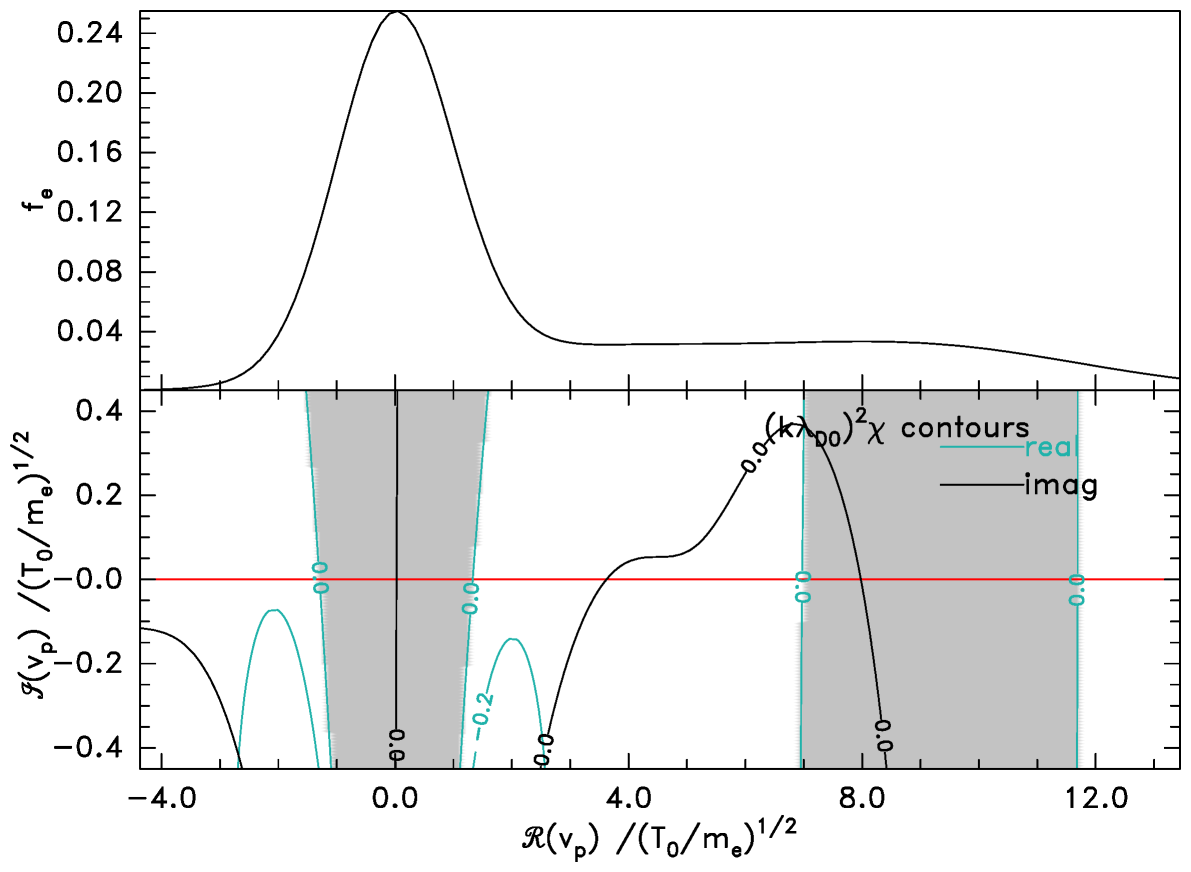
\includegraphics[width=.7\hsize]{eamode2}
  \caption{Unstable electron-acoustic mode ignoring ion response.}
  \label{fig:eamode2}
\end{figure}

\appendix
\section{Group Velocity}

The plots automatically give the phase velocity of the wave, since
they are plots on the real and imaginary axes of $v_p$. The group
velocity corresponding to waves on these solution contours can be
found as follows.
\begin{equation}
  \label{vgroup}
  v_g = {d\omega\over dk} = {d\over dk}(v_p k) = v_p + {k\over
    dk/dv_p} = v_p + {k\lambda_{D}\over d(k\lambda_{D})/dv_p}
\end{equation}

We substitute the value $k^2\lambda_{D}^2$, from eq.\
(\ref{ksquared}), which is what is contoured in the plots. And we
recognize that the second term by which $v_g$ differs from $v_p$ is
simply half the scale length of the variation of $k^2\lambda_{D}^2$ as
a function of $v_p$. Since (except for the zero level) the contours
are logarithmic in the ratios 1,2,5, the distance between the
function's contours is approximately the scale length of the function.


Therefore the value of the group velocity is approximately half way
between the contour of $-\Re (k^2\lambda_{D}^2 \chi_i)$ on which
it lies and the adjacent contour further from the shaded boundary. In
most cases the shift from $v_p$ is small enough to be inconsequential.
There will be zero group-velocity solutions only if there are
solutions with nearly zero phase velocity.

\end{document}

%%% Local Variables:
%%% mode: latex
%%% TeX-master: t
%%% End:
